\documentclass{fancyArticle}

\checkandfixthelayout

%% Define the labels for different environments for autoref
\def\propautorefname{Proposition}
\def\corollaryautorefname{Corollary}
\def\lemautorefname{Lemma}
\def\theoremautorefname{Theorem}
\def\equationautorefname{Equation}
\def\sectionautorefname{Section}
\def\figureautorefname{Figure}
%% Custom commands
\providecommand{\E}{\symcal{E}}             % Experiment label
\providecommand{\I}{\symfrak{I}}            % Imaginary part
\providecommand{\P}{\symbb{P}}              % Probability
\providecommand{\EV}{\symbb{E}}             % Expectation
\renewcommand{\|}{\,|\,}                    % spaced conditional bar
\providecommand{\;}{\,;}                    % spaced semicolon
\renewcommand{\O}{\symit{O}\:\!}            % Big O

\title{\large Consumer theory for cheap information}
\author{\textsc{Gary Baker}}
\date{This version: \today}

\begin{document}
\maketitle
\begin{center}
  \href{https://www.garygbaker.com/info-consumer-theory.pdf}{\color{blue}
    \underline{\textsc{click here for the most recent version}}}
\end{center}

\begin{abstract}
  Classic comparisons---e.g. Blackwell efficiency---of information sources tell us little about tradeoffs between different sources, especially when they differ in cost.
  %
  This paper seeks to fill that gap for finite-state environments by describing the consumer theory of information when information is cheap (or budgets large).
  %
  Motivated by large deviations theory, I propose a generalized notion of precision that measures how well an information source distinguishes two possible states.
  %
  I then show that maximizing the precision of the worst-case state pair yields an approximation for information demand with percent error vanishing proportionally with costs.
  %
  I further show iso-least-precision sets have finitely many kinks and are otherwise bowed \textit{out},
  and thus information demand exhibits vanishing substitution effects at almost all cost ratios.
  %
  This kinked geometry additionally implies an upper bound on the number of information sources that will ever be used in non-vanishing proportions: at most as many as there are state pairs.
  %
  Finally, because precision is independent of prior and payoffs, all decision-makers roughly agree on the optimal bundle.
  %
  In sum, demand for information starkly deviates from the benchmark convex preferences model of standard consumer theory.\\

  \textsc{keywords:} Demand for information, value of information, Bayesian decision theory, comparison of experiments, large deviations theory
\end{abstract}


%%%%%%%%%%%%%%%%%%%%%%%%%%%%%%%%%%%%%%%%%%%%%%%%%%%%%%%%%%%%%%%%%%%%%%%%
%% Introduction
%%%%%%%%%%%%%%%%%%%%%%%%%%%%%%%%%%%%%%%%%%%%%%%%%%%%%%%%%%%%%%%%%%%%%%%%

\section{Introduction}
\label{sec:introduction}

Often a decision-maker may find herself in a position to acquire information prior to making a decision under an uncertain state of the world, and many cases, she must not only decide how much information to purchase, but also from where to acquire it.
For example, a reader of the news must every day decide both how long and from which news sites to read, or a researcher studying the effects of a new drug on a disease might have multiple available tests of differing cost for the disease.
With the explosive growth of the internet and the availability of not just near-unlimited quantities of information, but also information from highly varied and distinct sources, questions such as these are more relevant than ever.

In these scenarios, how might one determine the optimal bundle of information? Are corner solutions always optimal? And if not, when?

Answering these questions ought to be little more than a standard consumer theory exercise: set the marginal rate of substitution equal to the price ratio along a budget constraint.
Unfortunately, such an exercise presupposes understanding of a utility function---no mean feat when the value for information is notoriously ill-behaved.\footnotemark\
\footnotetext{%
  Most famously, value of information is often non-concave, and thus marginal value of information is often rising.
  See, for example \citep{Radner1984} or \cite{Chade2002}.}

I provide an answer to these questions for environments with finitely many possible underlying states, valid when information is sufficiently cheap (or budgets sufficiently large).

In particular, drawing on large-deviations methods, I define a generalized notion of \textit{precision} that measures how well an information source (Blackwell experiment) discriminates between a given pair of possible states (a dichotomy).
I then show that a maximin rule---maximize the total precision of the bundle for the worst-case state pair---yields an approximation for demand, with percent error vanishing proportionally with costs (\autoref{result:maximin}).
Furthermore, because precision is a purely statistical property, independent of prior and payoffs, all decision-makers roughly agree on the optimal bundle at low costs.

\begin{figure}[t]
  \centering
  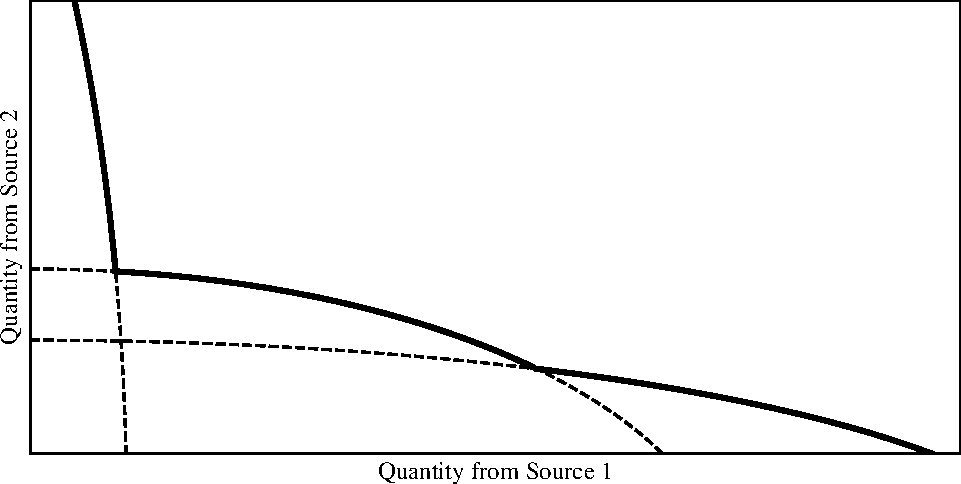
\includegraphics[width=0.85\textwidth]{figures/figqualitative.pdf}
  \caption{%
    An example geometry of iso-precision lines---and thus the approximate geometry of preferences---in a three-state environment with two available information sources.
    Iso-precision lines for a fixed dichotomy (dashed lines) bow out, but the iso-least-precision line (solid line) has inward pointing kinks.
  }\label{fig:example-ic}
\end{figure}

I then explore properties of demand by treating maximin precision \textit{as if} it were a utility function.
In particular, for a fixed-dichotomy precision is homothetic and iso-precision-lines bow \textit{out}---that is, precision of composite sources is less than the sum of its part---so iso-\textit{least}-precision lines exhibit inward-pointing kinks (\autoref{fig:example-ic}).

Maximin precision bundles thus only occur in finitely-many possible relative proportions (\autoref{result:complements}), corresponding with iso-least-precision corners and kinks, and thus demand for information behaves as if sources were perfect complements for small price changes, with large substitution effects only near costs where the maximin precision bundle jumps between kinks/corners.
Furthermore, homotheticity of precision guarantees all information sources have income elasticities approach unity, and thus no information source is ever an inferior good.

The kinked geometry additionally implies a relationship between the number of possible states number of information sources ever consumed in non-vanishing proportions (\autoref{result:complexity}).
As a consequence, at low costs, no decision-maker will ever consume more information sources (in non-vanishing proportions) than there are pairs of states.
Thus, in the simplest, two-state hypothesis testing world, only corners are ever optimal, with interior solutions only occurring with more complex decision problems.

Although the as-if-kinked nature of preferences would seemingly render discussion of the marginal rate of substitution away from the kinks pointless, information is not a typical good.
Data sets might have hard upper bounds on the number of available samples and the non-rival nature of information consumption often leads to non-linear (e.g. subscription) pricing schemes.
Such is to say: even with kinks, a complete consumer theory should describe the marginal rate of substitution elsewhere.
To that end, I show that, when the worst-case dichotomy is unique, the information from distinct sources is substitutable roughly in proportion to each source's \textit{marginal} precision (\autoref{result:mrs}).

This paper is most closely related to the work of \cite{Moscarini2002} who draw on large-deviations methods to write an approximation for information value, and thus information demand, in a quasilinear setting with one available source of information.
My \autoref{result:multi-ms02} generalizes their main result to a setting with multiple available sources and improves upon their estimate of the approximation's convergence rate.

Additionally, this result fits into the statistical literature on asymptotic relative efficiency, which traditionally asks how many samples from one statistical test are required to perform as well as a given number from another---that is, relative efficiency typically only considers the corners.
In particular, these results generalize Chernoff's \citeyearpar{Chernoff1952} notion of relative efficiency to a setting with multiple hypotheses (more than two states) and demonstrates the existence of non-corner solutions in such a setting.

These results lend themselves to multiple applications.
First and foremost, they provide a general approach for analysis of information markets, and suggest caution when dealing with information as a good in applied settings.
In particular, the benchmark consumer theory model (smooth, convex preferences) is fails rather starkly.

On a more practical note, the maximin precision rule also suggests a criterion for optimal experiment design, accounting not just for differing statistical properties of the different options, but also their costs.\footnotemark\
\footnotetext{%
  Experiment design is a large and varied statistical literature going back to Fisher (and arguably Gauss).
  For a textbook treatment, see \cite{Montgomery2012}.
  I consider experiment design implications more carefully in a separate working paper generalizing these results to certain regression settings.}

The remainder of this paper is structured as follows: \autoref{sec:model} lays out the formal model assumptions, including the relevant notion of information ``quantity'' used throughout this paper.
\autoref{sec:background} covers the necessary large-deviations background.
\autoref{sec:results} defines precision, states the maximin approximation rule, and explores features of the implied consumer theory.
Lastly, \autoref{sec:numerical} explores the performance of the approximations in practice.
Finally, \autoref{sec:conclusion} concludes.



%%%%%%%%%%%%%%%%%%%%%%%%%%%%%%%%%%%%%%%%%%%%%%%%%%%%%%%%%%%%%%%%%%%%%%%%
%% Model
%%%%%%%%%%%%%%%%%%%%%%%%%%%%%%%%%%%%%%%%%%%%%%%%%%%%%%%%%%%%%%%%%%%%%%%%

\section{Model}
\label{sec:model}

A decision-maker (DM) must choose an action~$a$ from a finite set,~$A$, under an uncertain state of the world~$\theta$ drawn from a finite set,~$\Theta$.
The DM has Bernoulli utility~$u(a, \theta)$ and a full-support prior~$p\in\Delta\Theta$.
For simplicity, assume the optimal action for each state, $a^{*}(\theta)\equiv\argmax_{a}u(a,\theta)$, is unique and distinct for all states.
The DM chooses her action to maximize expected payoffs.

Prior to acting, the DM may purchase information about the state of the world from $J$ distinct sources, $\E_1,\ldots,\E_J$.
Each information source is a conditionally independent Blackwell experiment,
$\E_{j} = \langle\mathbb{X}, \langle \mu_{j\theta}\rangle_{\theta\in\Theta}\rangle$, consisting of a collection of state-dependent distributions over some arbitrary space of realizations,~$\mathbb{X}$.
Assume each information source is informative, but no realization perfectly rules in or any strict subset of the world.
Formally, $\mu_{j\theta}$ and $\mu_{j\theta'}$ are mutually absolutely continuous and thus have defined likelihood ratios (Radon-Nikodym derivatives) $d \mu_{j\theta}/d \mu_{j\theta'}$.

Under this assumption, the $\mathbf{R}^{|\Theta|-1}$ vector of log-likelihood ratios  relative to some base state, $\theta_{0}$, is a sufficient statistic for each realization.
We can thus without loss of generality identify each realization by its own vector of log-likelihood ratios:
\begin{equation*}
  \mathbf{x}\equiv(x_{\theta})_{\theta\neq\theta_0}=\left(
    \log \left( {d \mu_{j\theta} \over d \mu_{j\theta_{0}}}(\mathbf{x}) \right)
  \right)
\end{equation*}
Because Bayes's rule is a sum when expressed in terms of log-likelihood ratios, we thus can summarize conditionally independent realizations from multiple sources simply by adding their log-likelihood ratios.
To avoid technicalities, assume all log-likelihood ratio distributions are thin-tailed in the sense that they have well-defined moment-generating functions on an open set containing the origin.

The DM chooses a \textit{quantity}, $\mathbf{t}=(t_1,\ldots,t_{J})\in\mathbb{R}^{J}$, of information from each information source at costs, $\mathbf{c}=(c_1, c_2, \ldots, c_J)=(\varepsilon,\varepsilon \kappa_{2},\ldots,\varepsilon \kappa_J)$ per unit quantity from each source subject to budget constraint, $Y$.
The key approximation will hold as costs become small, which I capture by setting $\varepsilon$ to be small.

Quantity of information is usually measured by conditionally i.i.d. samples---a fundamentally discrete object, but
to avoid discrete-optimization technicalities, I will assume for exposition\footnotemark\ that sources are \textit{infinitely divisible}.
\footnotetext{All results hold when quantity is measured by non-divisible samples. See Appendix \ref{sec:discrete}.}
Formally, $\E$ is infinitely divisible if for any $k$, there exists an experiment $\E^{1/k}$ such that $k$ conditionally i.i.d. samples from $\E^{1/k}$ are equivalent to a single sample from $\E$.

Thus, a rational quantity $t_j=a/b$ of information from $\E_j$ is equivalent to $a$ conditionally i.i.d. samples from $\E^{1/b}_j$.
Formally, the state-$\theta$ log-likelihood ratio distribution of rational quantity $t=n/k$ of $\E_{j}$, $\mu_{j\theta}^t$, is $\bigstar_{i=1}^{n}\mu_{j\theta}^{1/k}$, i.e. the $n$-fold convolution\footnotemark\ of the log-likelihood ratio distribution of $\E^{1/k}$.
\footnotetext{%
  $(\mu_1 \star \mu_2)(S) \equiv \int \mathbf{1}_{S}(x+y) \mu_1(dx)\mu_2(dy)$, i.e. the distribution of the sum.}
Non-rational quantities are simply the appropriate limit---for example, the sum of the appropriate number of samples from $\E_j^{1/10}$, $\E_j^{1/100}$, and so on.\footnotemark\
\footnotetext{Theorem 3, Chapter 9 of \cite{LeCam1986} guarantees that such a limit is a valid experiment.}
Because the moment-generating function of a sum is simply the product of moment-generating functions, the quantity-$t$ conditional distributions of log-likelihood ratios are perhaps more easily described in terms of their moment-generating functions:
if the moment-generating function of $\mu_{j\theta}$ is $M_{j\theta}(\zeta)$, then the moment-generating function of $\mu_{j\theta}^{t}$ is $M_{j\theta}(\zeta)^{t}$.

We can equivalently view quantity of information as a time spent observing a continuous-time, state-dependent process with conditionally independent increments.\footnotemark\
\footnotetext{%
   See Theorem 2.IX.5 of \cite{Feller1970} for a proof of this claim.}
For example, a DM might choose how long to watch a given news channel, where state-dependent new stories arrive according to a (state-independent) Poisson process.
Given the ubiquity of time constraints, in my budget-constrained setting, time is perhaps the most natural interpretation; however, remember the model is formally static: the DM chooses quantity, then observes the realizations all at once.

After choosing an information bundle, the DM observes the realizations, Bayes updates her beliefs appropriately, and chooses an action to maximize her expected payoff.
The DM thus wants to choose the feasible bundle that minimizes her expected loss\footnotemark\ from acting after observing the realizations:
\footnotetext{%
  Equivalent to maximizing the usual value of information in a budget-constrained setting.}
\begin{equation}\label{eq:expected-loss}
  L(\mathbf{t}) = \sum_\theta p_\theta \int_{\mathbf{x}\in \mathbb{R}^{|\Theta|-1}}
  \big(u(a^*(\theta),\theta) - u(a(\mathbf{x}),\theta)\big)
  \mu_{\theta}^{\mathbf{t}}(d\mathbf{x})
\end{equation}
where $a(\mathbf{x})$ is the expected-payoff-maximizing decision\footnotemark\ after observing realized log-likelihood ratios $\mathbf{x}$, and $\mu_{\theta}^{\mathbf{t}}$ is the log-likelihood ratio conditional distribution of realizations for the chosen expected sample bundle,  $\mu_{\theta}^{\mathbf{t}} \equiv \bigstar_{j=1}^J \ \mu_{j\theta}^{t_j}$.
\footnotetext{%
  Although for simplicity, I work with a Bayesian optimal decision rule---i.e. the DM uses the optimal decision thresholds for a log-likelihood ratio test---similar to \cite{Chernoff1952}, my approach applies for general decision rules based on additive statistical test under suitable regularity conditions.
  }

Except under restrictive functional-form assumptions on the available information sources, \autoref{eq:expected-loss} has no convenient closed form, necessitating the application of a large-sample approximation.


%%%%%%%%%%%%%%%%%%%%%%%%%%%%%%%%%%%%%%%%%%%%%%%%%%%%%%%%%%%%%%%%%%%%%%%%
%% Large deviations
%%%%%%%%%%%%%%%%%%%%%%%%%%%%%%%%%%%%%%%%%%%%%%%%%%%%%%%%%%%%%%%%%%%%%%%%

\section{Large deviations}
\label{sec:background}

Because large-deviations methods are relatively uncommon in economics, I will introduce the approach first in the two-state/two-action world.
Here we can pose the decision problem as a classic statistical dichotomy: there are two states $\Theta = \{\theta_0,\theta_1\}$, corresponding with \textit{null} and \textit{alternative} hypotheses, and the DM must either choose to \textit{reject} ($a= \mathcal{R}$) or \textit{accept} ($a= \mathcal{A}$) the null.
Naturally, the DM wants to reject when the null is false and vice-versa so the payoffs satisfy $u(\mathcal{R},\theta_1)>u(\mathcal{A}, \theta_1)$ and $u(\mathcal{A},\theta_0)>u(\mathcal{R},\theta_{0})$.
Assume the DM has prior $p$ that the alternative ($\theta_1$) is true, and the belief that makes the DM exactly indifferent between the two actions as $\bar{p}$.

Following \cite{Moscarini2002}, we can write the expected loss from quantity $\mathbf{t}$ in this environment in terms of the Type-I and Type-II error probabilities (respectively, $\alpha_{I}$ and $\alpha_{II}$):
\begin{equation*}
  \label{eq:2state-loss}
  L(\mathbf{t}) =
  (1-p) \alpha_{I}(\mathbf{t}) (u(\mathcal{A},\theta_0) - u(\mathcal{R},\theta_0))
  +
  p \alpha_{II}(\mathbf{t}) (u(\mathcal{R},\theta_1) - u(\mathcal{A},\theta_1))
\end{equation*}
As the quantity of information gets large, the error probabilities should fall to zero.
With a single source of information we can write the Type-I error probability, leveraging the fact that Bayes's rule is a sum when written in terms of log-likelihood ratios:
\begin{equation}
  \label{eq:type-i}
  \alpha_I(t) = \mathbb{P}\left(
  l + s_t > \bar{l} \| \theta_0\right)
\end{equation}
where $l=\log(p/(1-p))$ is the prior log-likelihood ratio, $\bar{l}=\log(\bar{p}/(1-\bar{p}))$ is the log-likelihood ratio of the indifference belief, and $s_t$ is the log-likelihood ratio of the realization of quantity $t$ of information.
Note that the expected value of the log-likelihood ratio when $\theta_{0}$ is true must be negative---i.e. when $\theta_0$ is true, on average the realizations should push the log-likelihood posterior \textit{down} towards stronger beliefs that $\theta_0$ is true.

Notice we could have equivalently written \ref{eq:type-i} in terms of the sample average log-likelihood ratio as follows:
\begin{equation*}
  \alpha_I(t) = \mathbb{P}\left(
    \frac{s_t}{t} > \frac{\bar{l}-l}{t} \ \bigg|\  \theta_0\right)
\end{equation*}
Here we can see why we can't use a more familiar asymptotic approach such as a central limit theorem: $\EV(s_t/t)\equiv \bar{s}<0$ but mistakes happen roughly only when the sample average is positive---i.e. \textit{far} from its mean.
This contrasts with the central limit theorem which describes the distribution of a sample average \textit{near} the mean (roughly, within $1/\sqrt{t}$ of the mean).

\cite{Cramer1938} canonically showed that the probability of such a large deviations is falling exponentially fast with rate given by a minimized moment-generating function.
We can see a basic version of this by an application of Markov's inequality:
\begin{equation*}
  \label{eq:chernoff-inequality}
  \alpha_I(t)
  \approx
  \mathbb{P}\left(
    \frac{s_t}{t} > 0 \ \bigg|\  \theta_0\right)
  =
 \mathbb{P}\left(
    \exp \left(\zeta \frac{s_t}{t} \right) > 1 \ \bigg|\  \theta_0\right)
  < {\min_{\zeta}\{M(\zeta)\}}^t
\end{equation*}
where $M$ is the state-$\theta_0$ log-likelihood ratio moment-generating function for a single unit of information.
Motivated by this approach, we can then turn back to the general finite-state problem.

Define the \textit{efficiency index}\footnotemark\ of  information source $\E_{j}$ for the $\theta,\theta'$ dichotomy as the minimized value of the moment-generating function for the $\theta,\theta'$ log-likelihood ratio conditional on true state $\theta'$:
\footnotetext{%
  I follow \cite{Moscarini2002} here.
  \cite{Torgersen1991} refers to this as the \textit{Chernoff number}.}
\begin{align*}
  \rho_j(\theta,\theta') \equiv \min_\zeta M_j(\zeta\,;\, & \theta,\theta')
                                  = \min_\zeta \left\{
                                  \int_{\mathbf{x}\in\mathbb{R}^{|\Theta|-1}}
                                  {\mu_{j\theta}(d\mathbf{x})}^{\zeta} {\mu_{j\theta'}(d\mathbf{x})}^{1-\zeta}
                                  \right\}
                                  \label{eq:hellinger}
\end{align*}
Note that $\rho_j(\theta,\theta')=\rho_j(\theta',\theta)$ because $M_j(\zeta\,;\,\theta,\theta')=M_j(1-\zeta\,;\,\theta',\theta)$ so the index is unique for a given dichotomy, independent of order.
This efficiency index---a special case of the index developed by \cite{Chernoff1952} for evaluating the asymptotic relative efficiency of two statistical tests---describes the exponential rate at which the Type-I or Type-II error problems fall in a simple testing problem.
Efficiency indices are always between 0 and 1 and are multiplicative for i.i.d. samples.
Furthermore, \textit{lower} efficiency index indicate \textit{better} large sample performance.\footnotemark
\footnotetext{%
  If $\E_1$ Blackwell dominates $\E_2$ then $\E_1$ has lower efficiency indices for all dichotomies.}

Unlike the previous literature, however, I am not just interested in the behavior of individual information sources in isolation, but also how they interact when used together.
To generalize the efficiency index to a setting with multiple sources, first denote the total quantity, $T \equiv \sum t_j$ and the proportions of total quantity from each experiment as $\mathbf{r} = (r_1,\ldots,r_J) \equiv (t_1/T,\ldots,t_j/T)$.

Then define the $\mathbf{r}$-composite experiment as one with quantities $\mathbf{r}$ from each information source.
This constructed source then has log-likelihood rate moment-generating functions, $M_{\mathbf{r}}(\zeta;\theta,\theta')\equiv \prod M_j(\zeta;\theta,\theta')^{r_j}$.
By construction, quantity $T$ from the $\mathbf{r}$-composite experiment is equivalent to the bundle $\mathbf{t}$ because $M_{\mathbf{r}}^T=\prod M_j^{t_{j}}$.
Define the \textit{composite} efficiency index $\rho_{\mathbf{r}}(\theta,\theta')$ analogously.
\begin{equation*}
  \label{eq:composite-efficiency-index}
  \rho_{\mathbf{r}}(\theta,\theta') \equiv \min_{\zeta} \left\{
  \prod_{j=1}^{J} M_j(\zeta;\theta,\theta')^{r_j}\right\}
\end{equation*}

We can then further break $\rho_{\mathbf{r}}$ into contributions from each source by defining the \textit{marginal} efficiency index of $\E_j$ as $\rho_{j \mathbf{r}}(\theta,\theta')\equiv M_j(\zeta^{*}_{\mathbf{r}};\theta,\theta')$ where $\zeta^{*}_{\mathbf{r}}$ is the minimizer of $M_{\mathbf{r}}(\cdot;\theta,\theta')$, so
\begin{equation*}
  \label{eq:marginal-efficiency indices}
  \rho_{\mathbf{r}}(\theta,\theta')=\prod\rho_{j \mathbf{r}}^{r_j}(\theta,\theta')
\end{equation*}

With only two states, \cite{Moscarini2002} show that each mistake probability, and thus the expected loss itself, is proportional to $\rho^{t}/\sqrt{t}$ for $t$ large.\footnotemark\
\footnotetext{\cite{Moscarini2002} don't assume infinite divisibility, so quantity for them is simply number of conditionally i.i.d. samples}
With more than two states, they further show that, because each mistake probability is exponentially falling, the expected loss is eventually dominated by the most likely mistake---that is, the \textit{largest} efficiency index.
Using marginal efficiency indices, I can now state a generalized version of their main result:

\setcounter{prop}{-1}
\begin{proposition}
  \label{result:multi-ms02}
  Let $\mathcal{D}$ be the collection of dichotomies.
  Then when the worst-case dichotomy, $\argmax_{D}\rho_{\mathbf{r}}(D)$, is unique, the expected loss from consuming quantities $\mathbf{t}=[t_{1},\ldots,t_J]$ from $\E_{1},\ldots,\E_{J}$ is\footnotemark
  \footnotetext{%
  Say a function, $f(x)$ is $O(x)$ as $x$ goes to zero, if there exists some positive constant function such that for $x$ small enough, $|f(x)|<Cx$}
  \begin{equation}
    \label{eq:multi-fig}
    L(\mathbf{t}) = A(\mathbf{r}) \frac{\max\textstyle_{D\in \mathcal{D}}
      \big\{\prod\textstyle_{j=1}^J \rho_{j\mathbf{r}}{(D)}^{t_j}\big\}}
    {\sqrt{T}}
    \left( 1 + \O\left( \frac{1}{T} \right) \right)
  \end{equation}
  where $A(\mathbf{r})$ depends only on the relative proportions of each information source.
\end{proposition}
\begin{proof}
  See Appendix \ref{sec:proof-multi-ms02}.
  \renewcommand{\qedsymbol}{}
\end{proof}

A version of \autoref{result:multi-ms02} follows by direct application of Theorems 1 and 4 of Moscarini and Smith (with slight modification to allow for infinite divisibility); however, such would give a $\O(T^{1/2})$ remainder.
By contrast, I apply a different proof technology---a saddlepoint approximation due to \cite{Lugannani1980}---to show that the remainder is actually the tighter $O(T^{-1})$.

It's worth emphasizing that, efficiency indices are purely properties of the information sources, not the decision maker's prior or payoffs.
Thus, at large enough quantities, all decision makers agree that an additional small $\delta$ from $\E_j$ reduces expected losses by a roughly factor of $\rho_{j\mathbf{r}}(D)^{\delta}$.

Note that from \autoref{result:multi-ms02} we immediately get a multi-state generalization of the main result of \cite{Chernoff1952} for log-likelihood ratio tests.

\begin{corollary*}[Chernoff's asymptotic relative efficiency]
  If $\E_1$ and $\E_2$ are two information sources with efficiency indices $\rho_1(\cdot)$ and $\rho_2(\cdot)$ respectively, then if quantity $t_1$ from $\E_1$ has the same expected loss as $t_2$ from $\E_2$ then, for\ \ $t_1$ large
  \begin{equation*}
    \label{eq:chernoff-are}
    \frac{t_2}{t_1} \approx
    \frac{\log(\max_{D\in \mathcal{D}}\{\rho_1(D)\})}
    {\log(\max_{D\in \mathcal{D}}\{\rho_2(D)\})}
  \end{equation*}
\end{corollary*}

The above result illustrates the importance of the \textit{log} efficiency index for substitutability of different sources, but tells us little about preferences away from the corners.
Of course, this would be sufficiency to characterize demand if corners were always optimal, but as we'll shortly see, interior solutions are quite common.

To get a complete consumer theory, we need to take a closer look at the approximation given by \autoref{result:multi-ms02}.

%%%%%%%%%%%%%%%%%%%%%%%%%%%%%%%%%%%%%%%%%%%%%%%%%%%%%%%%%%%%%%%%%%%%%%%%
%% Results
%%%%%%%%%%%%%%%%%%%%%%%%%%%%%%%%%%%%%%%%%%%%%%%%%%%%%%%%%%%%%%%%%%%%%%%%

\section{Results}
\label{sec:results}


%%%%%%%%%%%%%%%%%%%%%%%%%%%%%%%%%%%%%%%%%%%%%%%%%%%%%%%%%%%%%%%%%%%%%%%%
%% Precision and demand
%%%%%%%%%%%%%%%%%%%%%%%%%%%%%%%%%%%%%%%%%%%%%%%%%%%%%%%%%%%%%%%%%%%%%%%%

\subsection{Precision and information demand}\label{sec:demand}

Recall that the DM's objective is to \textit{minimize} the expected loss, but the multiplicative form of~\autoref{eq:multi-fig} begs to be transformed by logs.
Under a budget constraint, the DM will equivalently choose her information bundle to maximize $-\log(L(\mathbf{t}))$, so we can use such as ``utility'' for information. I thus denote $U(\mathbf{t})\equiv -\log(L(\mathbf{t}))$.

Define the \textit{precision} of an information source as
\begin{equation*}
  \label{eq:precision-definition}
  \beta_{j}(D) \equiv -\log(\rho_{j}(D))
\end{equation*}
Similarly, define the marginal precision $\beta_{j\mathbf{r}}(D)=-\log(\rho_{j\mathbf{r}}(D))$.
Since $\beta$ is additive for i.i.d. samples and higher for more informative (lower efficiency index) experiments, one can view it as a generalization of the classic notion of precision.
In fact, for a standard Gaussian signal which reveals the true state plus mean-zero noise with variance $1/\gamma$---that is, with (classical) precision $\gamma$---the generalized precision is proportional to $\gamma$.

Using \autoref{result:multi-ms02} we can then write utility for information as
\begin{equation}
  \label{eq:info-utility}
  U(\mathbf{t}) = \min_{D\in D}\left\{ \sum_{j=1}^J t_j \beta_{j \mathbf{r}}(D) \right\}
  \left( 1 + O\left(\frac{\log(T)}{T}\right) \right)
\end{equation}

That is, at large quantities, the DM prefers bundles with higher total precision for their \textit{worst-case} dichotomy.
The following proposition guarantees the stronger claim that the maximin precision bundle is close to the true optimal, loss-minimizing one:

\begin{proposition}[Maximin precision]\label{result:maximin}
  As all costs go to zero ($\varepsilon \rightarrow 0$), the loss-minimizing information bundle is $\mathbf{t}^{*} = \bar{\mathbf{t}}(1+O(\varepsilon))$
  where $\bar{\mathbf{t}}$ maximizes the worst-case total precision, $\min_D\sum t_j\beta_{j \mathbf{r}}(D)$, subject to $\mathbf{c} \cdot \mathbf{t}\leq Y$.
\end{proposition}
\begin{proof}
  Making costs ($\varepsilon$) small is equivalent to making the budget large, so fix sample cost vector $\mathbf{c}$.
  Let $\mathbf{r}^{*}_{Y}$ be the relative proportions of the loss-minimizing bundle at budget $Y$ and $\bar{\mathbf{r}}$ the same for the least-precision per dollar bundle (not necessarily unique).
  Then we must have
  \begin{equation*}
    \underline{A}
    \frac{\max\textstyle_{D}
      \left\{\rho_{\symbf{r}^{*}_Y}{(D)}^{Y/(\mathbf{r}^{*}_Y\cdot c)}\right\}}
    {\sqrt{Y/(\mathbf{r}^{*}_Y\cdot c)}}
    <
    \overline{A}
    \frac{\max\textstyle_{D}
      \left\{\rho_{\mathbf{r}^{*}}{(D)}^{Y/(\mathbf{r}^{*}\cdot c)}\right\}}
    {\sqrt{Y/(\mathbf{r}^{*}\cdot c)}}
  \end{equation*}
  where $\overline{A}<\infty$ and $\underline{A}>0$ are upper and lower bounds on $L(\mathbf{t})(\max_{D} \rho_{\mathbf{r}}(D)^T)^{-1} \sqrt{T}$ for $T\geq 1$ (shown to exist, even when the worst-case dichotomy is non-unique, in Appendix \ref{sec:proof-maximin}).
  Taking logs and rearranging terms we have that the precision per dollar at the true optimal proportions approaches the maximal least-precision per dollar at rate $\O(Y^{-1})$.
  Application of Taylor's theorem completes the proof, because precision is differentiable in $\mathbf{r}$ for each dichotomy.
  Technical details are deferred to Appendix \ref{sec:proof-maximin}.
  \renewcommand{\qedsymbol}{}
\end{proof}

In short, \autoref{result:maximin} allows us to analyze preferences over information bundles by treating worst-case total precision \textit{as though} it were the DM's utility function.

Interestingly, this implies that our risk-neutral DM behaves as though she were extremely risk-\textit{averse}---choosing her information bundle to minimize the probability of the most likely mistake.
Further, because precision is independent of DM specifics, whenever the maxi-min precision is unique, all DMs will agree on the optimal bundle, up to a vanishing (percent) remainder.

By this approach, we can see that information demand will have some peculiar properties following from the unusual nature of least total precision. For example, the following lemma implies low-cost information demand deviates starkly from the benchmark differentiable, quasiconcave utility model:

\begin{lemma}[Properties of precision]\label{result:local-convexity}
  For a fixed dichotomy, precision is homothetic and quasiconvex in quantity, $\mathbf{t}$.
  The worst-case total precision is thus homothetic and\, \textup{locally} quasiconvex\footnotemark\ around any bundle where the least-precision dichotomy is unique.
  \footnotetext{Say a function is \textit{locally quasiconvex} at $\mathbf{t}$ if, for a small enough open ball, the intersection of the lower contour set of $\mathbf{t}$ and the ball around $\mathbf{t}$ is convex.}
\end{lemma}

\begin{proof}
  Homotheticity follows immediately: scaling up an information bundle does not change the relative proportions of each information source in the bundle, and thus does not affect marginal precisions.
  To see quasiconvexity, recall that $\rho_{j \mathbf{r}}(D)$ is the moment-generating function for the $D$-dichotomy log-likelihood ratio evaluated at the minimizer for the whole bundle.
  We thus have for a fixed dichotomy, $\prod {\rho_{j \mathbf{r}}(D)}^{r_j} \geq \prod {\rho_j(D)}^{r_j}$, or equivalently
  \begin{equation}\label{eq:prec-convex}
    \sum_{j=1}^J r_j\beta_{j \mathbf{r}}(D) \leq \sum_{j=1}^J r_j \beta_{j}(D)
  \end{equation}
  (with equality if and only if all sources with $r_{j}>0$ have the same log-likelihood ratio moment-generating function minimizer).
  Put another way, precision of a bundle is less than the sum of its parts for a fixed dichotomy.
  Minimization does not preserve quasiconvexity, but because there are only finitely-many dichotomies, local behavior is preserved around any point where the worst-case dichotomy is unique (typically almost everywhere).
  \renewcommand{\qedsymbol}{}
\end{proof}

\autoref{result:local-convexity} has two important implications.
First, homotheticity implies optimal proportions, $\mathbf{r}$, are income-independent, so we can equivalently solve the maximin precision problem by finding proportions that maximize the worst-case precision \textit{per dollar}, $\beta_{\mathbf{r}} / \mathbf{c} \cdot \mathbf{r}$.
Put another way, at low enough prices, there's no such thing as an inferior or luxury source of information:
\begin{corollary*}[Unit income elasticity]
  If the maximin precision per dollar bundle is unique, the arc\footnotemark\ income elasticity of demand for all information sources given a fixed change in income is $1+O(\varepsilon)$ as costs go to zero.
  \footnotetext{Differentiating $\O$ terms is only possible under limited circumstances---hence, the use of the arc formula.}
\end{corollary*}

Second, the local quasiconvexity imply that most information bundles cannot be optimal with a linear budget.
One would be forgiven for thinking \ref{eq:prec-convex} simply implies that loss-minimizing bundles must lie near corners; however, because only the least-precision dichotomy matters for big bundles, total \textit{least} precision will be non-quasiconvex whenever different sources have different worst-case dichotomies.
Intuitively, interior solutions may arise because distinct information sources can cover for the others' weaknesses.
In fact, so long as the information sources differ in their worst case dichotomy, interior solutions may arise even when one source has higher precision for \textit{all} dichotomies (or even more strongly, is Blackwell-dominant).%
\footnote{See the supplementary material for an example.}

The nature of these interior solutions is perhaps easiest understood geometrically by treating iso-least-precision curves as though they were the DM's indifference curves.
The iso-precision curve for each fixed dichotomy bows out, but the iso-\textit{least}-precision curve (the outer contour) will have inward pointing kinks when the worst-case dichotomy is non-unique (\autoref{fig:example-ic}).

We thus clearly have that for a generic pair of sources (whose iso-precision lines strictly bow out), information will be consumed in at most finitely many possible ratios corresponding with the corner solutions and kinks where iso-precision lines intersect.
\autoref{result:complements} generalizes this observation to generic, finite collections of information sources.

\begin{proposition}[Iso-least-precision kinks]\label{result:complements}
  For generic information sources---i.e. ones for which \ref{eq:prec-convex} holds strictly---across all costs, there are finitely many relative proportions, $\mathbf{r}$, that maximize worst-case precision per dollar, $\min_{D}\sum r_j\beta_{j \mathbf{r}}(D)/(\mathbf{c} \cdot \mathbf{r})$, and at almost all costs, the maximin-precision-per-dollar proportions are unique and invariant to small cost changes.
\end{proposition}
\begin{proof}[Proof (sketch)]
  Almost-everywhere local quasiconvexity guarantees that maximin precision guarantees that maximin precision proportions can only occur on a measure-zero set.
  Showing that only finitely many proportions are ever optimal is left to Appendix \ref{sec:proof-complements}.
  \renewcommand{\qedsymbol}{}
\end{proof}

Because interior maximin precision bundles are always at iso-least-precision kinks, information from different sources are locally perfect complements.
For small enough price changes, the change in demand is purely income effect: information sources are locally perfect complements.
\begin{corollary*}[Price elasticities]
  If the maximin precision bundle is unique (true for almost all cost vectors), the (arc) price elasticity of demand for all sources given a small enough percent change, $\delta$, of $c_i$ is
  $( r_{i}c_i / \mathbf{r} \cdot \mathbf{c} )\left( 1 + O \left( \varepsilon + \delta \right) \right)$
\end{corollary*}
However, around costs where the maximin precision is non-unique, information demand exhibits massive substitution effects as the demands jumps between kinks/corners.

%%%%%%%%%%%%%%%%%%%%%%%%%%%%%%%%%%%%%%%%%%%%%%%%%%%%%%%%%%%%%%%%%%%%%%%%
%% Number of Sources ever demanded
%%%%%%%%%%%%%%%%%%%%%%%%%%%%%%%%%%%%%%%%%%%%%%%%%%%%%%%%%%%%%%%%%%%%%%%%

\subsection{Complexity of optimal sample bundles}
\label{sec:complex-bundles}

Because iso-precision lines bow out, in the simplest, binary state, decision problems optimal information bundles only have a single information source (in non-vanishing proportions) at low costs.
Interior solutions can only occur in environments with at least three possible states.
This suggests that ``sophisticated'' bundles (more distinct sources) require more ``complicated'' decision problems (more possible states of the world).

In fact, because of the kinked geometry of the maxi-min precision problem,  there is a sharp relationship between the number of distinct information sources in a bundle and the number of dichotomies:

\begin{proposition}\label{result:complexity}
  If proportions\ \,$\mathbf{r}^{*}$ maximize the worst-case precision per dollar and has support on\ $K$ distinct generic information sources, then the\ \,$\mathbf{r}^{*}$-composite experiment has equal precision for at least\ (generically, exactly) $K$ dichotomies.
\end{proposition}

\begin{proof}[Proof (sketch)]
  By \autoref{result:complements}, interior maxi-min precision bundles occur at kinks where multiple dichotomies have equal precision.
  If $\mathbf{r}^{*}$ has support on $K$ distinct sources, this kink must be $K$-dimensional, and thus be the intersection of $K$ iso-precision surfaces.
  See Appendix \ref{sec:proof-complexity} for a formal proof.
  \renewcommand{\qedsymbol}{ }
\end{proof}

We can thus put an upper bound on the number of information sources that will ever be consumed in non-vanishing proportions at large budgets: at most as many as there are dichotomies ($|\Theta|(|\Theta|-1)/2$).

\subsection{Tradeoffs between sources of information}\label{sec:tradeoffs}

In the linear-constraint setting, the kinked nature of solutions renders the marginal rate of substitution between sources effectively irrelevant.
However, information is a peculiar good, and non-linear costs arise quite naturally.
For example, data sources will have a fixed upper bound on available samples (at least in the short term).
Further, the non-rival nature of information consumption lends itself to non-linear pricing schemes such as subscriptions and bundling.

In such cases, the maxi-min precision solution might not be feasible, and the marginal rate of substitution might prove useful.

\autoref{eq:info-utility} suggests that, provided the worst-case dichotomy is locally unique, the marginal utility for information from a given source ought to be roughly to that source's marginal precision.
Thus sources should be roughly substitutable in proportion to their relative marginal precision.
Normally, however, we should be cautious of heuristics that rely on differentiating $\O$ terms.

Fortunately, a variation of the same saddlepoint method used to prove the expected loss approximation \autoref{result:multi-ms02} works equally well to on the derivative of expected loss:
\begin{proposition}[Marginal rate of substitution]\label{result:mrs}
  At any bundle with unique worst-case dichotomy, $D$, the marginal rate of substitution between them is
  \begin{equation*}
    \frac{\partial L / \partial t_{1}}{\partial L / \partial t_{2}}
    = \frac{\beta_{1\mathbf{r}}(D)}{\beta_{2\mathbf{r}}(D)} + \O(T^{-1})
  \end{equation*}
\end{proposition}
\begin{proof}
  See Appendix \ref{sec:proof-mrs}.
  \renewcommand{\qedsymbol}{}
\end{proof}




%%%%%%%%%%%%%%%%%%%%%%%%%%%%%%%%%%%%%%%%%%%%%%%%%%%%%%%%%%%%%%%%%%%%%%%%
%% Numerical performance
%%%%%%%%%%%%%%%%%%%%%%%%%%%%%%%%%%%%%%%%%%%%%%%%%%%%%%%%%%%%%%%%%%%%%%%%

\section{How well does the approximation perform in practice?}
\label{sec:numerical}

It's worth considering whether any of these approximations are even useful in practice.
After all, in principal, the approximation holds only when information purchases are large, and thus when error probabilities are vanishingly small.
In such a world, does it really matter whether or not the DM chooses a bundle of information optimally?
I claim that, despite this, these approximations are still useful for understanding preferences.
To that end, I briefly discuss both the theoretical and numerical performance of these results.

\subsection{Theoretical performance}
\label{sec:theoretical-performance}

First, recall that these approximations have percent errors falling proportional with $1/T$, a respectable convergence rate by asymptotic approximation standards.
By comparison, the central limit theorem---a staple for estimating standard errors in applied work---converges with error falling with rate $1/\sqrt{T}$.
Although these approximations are not substitutes, based on convergence rates alone, the large deviations approach should be no more suspect than the central limit theorem one.

Second, from a practical standpoint, even though mistakes are very rare, they are an astronomically more rare when using the maximin precision rule:
\begin{corollary*}
  Let\, $\mathbf{t}^{*}(Y)$ be the maximal bundle with proportions\,  $\mathbf{r}^{*}$ maximizing worst-case precision per dollar and\, $\mathbf{t}(Y)$ be the same but for some other fixed proportions\, $\mathbf{r}$.
  Then the loss satisfies
  \begin{equation*}
   \lim_{Y\rightarrow\infty} \frac{L(\mathbf{t}(Y))}{L(\mathbf{t}^{*}(Y))} = \infty
  \end{equation*}
  where $Y^{*}$ is the required budget from purchasing information in proportions $\mathbf{r}^{*}$ and $Y$ the required budget purchasing in proportions $\mathbf{r}$.
\end{corollary*}

More strongly, this ratio not only grows without bound, but grows exponentially fast.
Thus, especially in environments where mistakes are extremely costly, choosing a bundle far from the maximin precision one can have extremely high costs.

\subsection{Numerical performance}
\label{sec:simulations}

We can't entirely justify these approximations by theory alone.
I conclude with a few observations of the approximation's performance in simulation.

\begin{figure}[t]
  \centering
 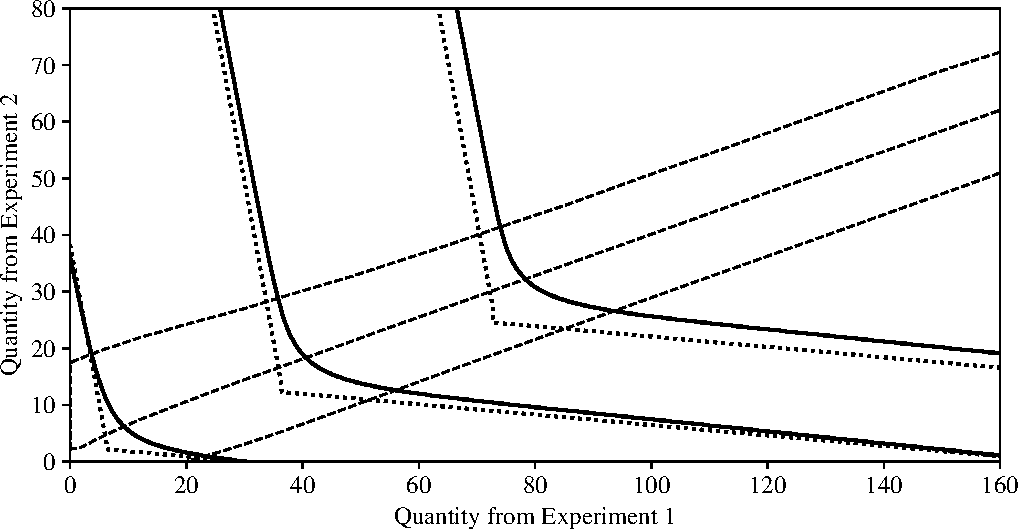
\includegraphics[width=0.85\textwidth]{figures/poissonincexp.pdf}
 \caption{%
   Illustration of income effects: income-expansion paths of demand in a three-state environment two two available sources of information.
   Dotted lines are the iso-least-precision lines, solid lines are numerically computed true indifference curves, and dashed lines are numerically computed true income expansion paths for three different cost ratios.
 }
  \label{fig:simulations}
\end{figure}

\autoref{fig:simulations} illustrates some of the main features of numerical simulations of information demand.\footnotemark
\footnotetext{%
  In these simulations, infinite divisibility is achieved by Poissonization. That is, instead of choosing number of samples directly, the DM chooses \textit{expected} samples and then receives a Poisson distributed draw of samples.}

First, recall that there are two main sources of approximation error: the pure large deviations error, and the error from ignoring all but the most likely mistake.
In theory, the error from ignoring less likely mistakes is exponentially falling and thus negligible in comparison to the $O(T^{-1})$ error of the large deviations approximation.
However, near iso-least-precision kinks, the second-most-likely mistake is nearly as likely as the most likely and thus the approximation performs comparatively poorly in those regions.\footnotemark
\footnotetext{%
  There is also a second order issue that because kinks point inward, total sample size tends to be lower than it would be at a corner on the same iso-precision-line.}
Graphically, this manifests as indifference curves taking a smooth curve rather than the sharp turn the iso-least-precision lines take.

This might seem like an issue given that optimal solutions are predicted to be at kinks, but because the approximation is very tight away from the kink, optimal bundles are still constrained to be near kinks.

The income expansion paths plotted in \autoref{fig:simulations} show this.
For high enough budgets, the true optimal bundle is within a constant (and thus vanishing percent error) of the kink.

\begin{figure}[t]
  \centering
  \begin{minipage}{0.45\linewidth}
    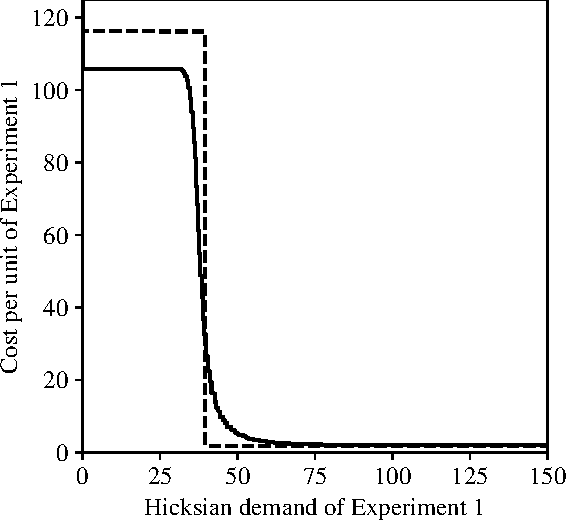
\includegraphics[width=\textwidth]{figures/hicksian1.pdf}
  \end{minipage}
  \hspace{2em}
  \begin{minipage}{0.45\linewidth}
    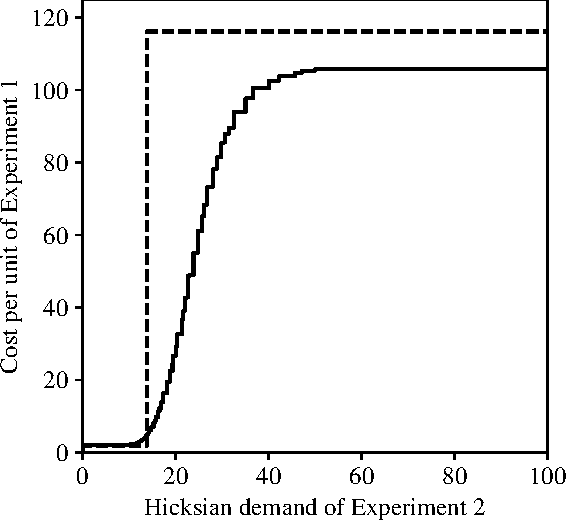
\includegraphics[width=\textwidth]{figures/hicksian2.pdf}
  \end{minipage}
  \caption{Illustration of substitution effects for information: Hicksian demand for the same information sources used in \autoref{fig:simulations} as a function of the cost of Experiment 1, holding the cost of Experiment 2 fixed. The solid line is a true Hicksian demand curve, and the dashed line is the equivalent curve predicted by the maximin precision rule.}
  \label{fig:hicksian}
\end{figure}

Even with these smooth curves around the kinks, demand still illustrates the predicted large substitution effects, jumping straight to the corners for steeper cost ratios.
To illustrate this, I plot in \autoref{fig:hicksian} a Hicksian (compensated)\footnotemark\ demand for information for the two information sources used in \autoref{fig:simulations}.
\footnotetext{%
  Hicksian demand holds expected losses constant rather than budget and thus illustrates demand absent any income effects.}
I use Hicksian, rather than the usual Marshallian, demand for two reasons. (1) the Hicksian demand predicted by the maximin precision rule takes a very simple form (a step function) and it is comparatively easy to visually evaluate the approximation quality,
and (2) by holding expected losses fixed, rather than budget, the quality of the approximation does not vary too much over the range of costs because total quantity does not vary much over the cost range as it would with a Marshallian demand curve.
Although the true Hicksian demand (solid) is not quite the step function predicted by the maximin precision rule (dashed line), it tracks very closely and illustrates the predicted small substitution effects everywhere except near the jump between kinks.

Finally, notice that even at low budgets when the approximation is poor on the \textit{intensive} margin, the maximin precision approximation typically performs well on the \textit{extensive} margin, correctly predicting the set of sources used in positive quantities.

All told, these results suggest that the approximations perform best when the number of states is relatively small, as many states can generate many kinks and thus may have relatively smooth, quasiconcave. indifference curves at realistic information quantities.

Interested readers can further explore the approximations for different sources of information in the simulations in the supplemental online materials.\footnotemark
\footnotetext{%
  Click \href{https://www.garygbaker.com/web-appendices/info-consumer-theory-discrete/}{\color{blue}\underline{here}}
  here to view the Jupyter noteboks.}



%%%%%%%%%%%%%%%%%%%%%%%%%%%%%%%%%%%%%%%%%%%%%%%%%%%%%%%%%%%%%%%%%%%%%%%%
%% Conclusion
%%%%%%%%%%%%%%%%%%%%%%%%%%%%%%%%%%%%%%%%%%%%%%%%%%%%%%%%%%%%%%%%%%%%%%%%

\section{Conclusion}
\label{sec:conclusion}

This paper has provided a general approach for understanding the consumer theory for information in finite-state/finite-action environments.
Specifically, using an improved version of the large-deviations approximation of \cite{Moscarini2002}, I have shown that information demand is, up to a percent error vanishing with costs, given by a maximin precision rule.

Notably, in contrast to a purely statistical approach to comparing information sources, my consumer-theoretic approach explicitly allowed consideration of costs and complementarities between different signals, and demonstrated the salience of interior solutions, typically neglected by the relative efficiency literature.

By treating worst-case precision as if it were utility, I was able to describe a variety of consumer-theoretic quantities of interest.
In particular, worst-case precision is kinked, and thus information demand behaves as if perfect complements at most costs.
Additionally, this approach allowed approximated the substitutability of different information sources whenever the worst-case dichotomy is unique.
Finally, the kinked nature of precision implied a novel relationship between the number of information sources used and the number of states: no more information sources will ever be consumed than there are state pairs.

These results ought to have application both to the economic theory of information, but also---more practically---to the optimal design of experiments.

All told, these results suggest caution when dealing with information as good: the standard assumptions (smooth, convex) fail rather spectacularly.



\begin{appendix}

  \pagebreak
  \section{Omitted proofs}
  \label{sec:proofs}

  %%%%%%%%%%%%%%%%%%%%%%%%%%%%%%%%%%%%%%%%%%%%%%%%%%%%%%%%%%%%%%%%%%%%%%%%
  %% MS02 saddlepoint proof
  %%%%%%%%%%%%%%%%%%%%%%%%%%%%%%%%%%%%%%%%%%%%%%%%%%%%%%%%%%%%%%%%%%%%%%%%

  \subsection{Proof of \autoref{result:multi-ms02}}
  \label{sec:proof-multi-ms02}

  Similar to \cite{Moscarini2002}, I start with the simple hypothesis testing problem with a single information source.
  That is, we have two states, $\theta_0$ and $\theta_1$, with prior that $\theta_1$ is true given by $p$, and two actions, accept and reject, where reject is optimal when $\theta_1$ is true.
  We can then write the expected loss as
  \begin{equation*}
    L(t) = (1-p)\alpha_I(t)L_I + p\alpha_{II}(t)L_{II}
  \end{equation*}
  where $L_I$ and $L_{II}$ are the ex-post losses from Type-I (rejecting when $\theta_0$ is true) and Type-II errors respectively, and $\alpha_I$ and $\alpha_{II}$ are the probabilities of those errors under a Bayesian decision rule.

  In this case, we can write the Type-I error probability as the probability the probability that the posterior log-likelihood ratio is above the rejection threshold when the true state is $\theta_0$:
  \begin{equation*}
    \alpha_{I}(n) = \mathbb{P}\left(
      \log \left( \frac{d\mu_{\theta_1}^t}{d\mu_{\theta_0}^t}(x) \right)
      > \bar{l} \ \bigg|\ \theta_0\right)
  \end{equation*}
  \cite{Moscarini2002} apply a classic change-of-measure approach similar to \cite{Cramer1938} to prove their main result for discretely sampled information sources, where the log-likelihood ratio is an i.i.d. sum.
  In contrast, I use a \textit{saddlepoint} approach which more cleanly applies to infinitely divisible source and gives a tighter bound on the approximation error:

  The saddlepoint approach roughly works by applying the method of steepest descents \citep[see Ch. 17][]{Jeffreys1956} to an inversion of the characteristic function.
  \cite{Daniels1954} first applied this approach using the classic inversion formula for a density, but our log-likelihood ratio doesn't necessarily have a density.
  So instead, I rely on an approximation due to \cite{Lugannani1980} who used a variation on the \cite{Gil-Pelaez1951} characteristic inversion formula:

  \begin{lemma*}[Characteristic function inversion]
    If\, $Y$ is a random variable with characteristic function $\phi$, then   the survivor function of\, $Y$ is
    \begin{equation*}
      \mathbb{P}(Y\geq y)
      = \frac{1}{2\pi}\int_{-\infty}^{\infty} \frac{e^{-iuy}\phi(u)}{iu}\D u
    \end{equation*}
    where the path of integration is perturbed to avoid the singularity at   the origin.
  \end{lemma*}

  We can then approximate the survivor function for the log-likelihood ratio by applying the method of steepest descents to its characteristic function:

  \begin{lemma*}[\citeauthor{Lugannani1980}, \citeyear{Lugannani1980}]
    Let\, $Y$ be a real-valued random variable with\, $\mathbb{E}(Y)<0$, and $\bar{Y}_n$ be the sample average of\, $n$ i.i.d. draws of\, $Y$.
    If\, $Y$'s characteristic function $\phi(\zeta)$, analytic through a strip, $\{\zeta:-\I(\zeta)\in(\zeta^{*}-\epsilon,\zeta^{*}+\epsilon)\}$, where\,   $\zeta^{*}\equiv\argmin_\zeta\mathbb{E}(e^{\zeta Y})$, then for\, $\xi$ close enough to zero
    \begin{equation}
      \label{eq:saddlepoint-cdf}
      \mathbb{P}(\bar{Y}_n\geq\xi) =
      \frac{e^{n(K(\zeta^{*}(\xi)) - \zeta^{*}(\xi) \xi)}}
      {\zeta^{*}(\xi) \sqrt{2\pi n K''(\zeta^{*}(\xi))}}
      \left(1+\O\left(\frac{1}{n}\right)\right)
    \end{equation}
    where\, $K(\zeta) \equiv \log(M(\zeta))$ is the cumulant generating function of\, $Y$ and\,  $\zeta^{*}(\xi)$ is the minimizer of\, $K(\zeta)-\zeta\xi$.
  \end{lemma*}
  Note that although \citeauthor{Lugannani1980} work with discretely sampled distributions, they use the method of steepest-descents to approximate the inversion given by the previous lemma, and thus works for any real-valued $n$, (though $\phi^{n}$ will only be a valid characteristic function when infinite divisibility applies).

  A reader interested in the logic of the proof should see the proof of \autoref{result:mrs} in Appendix \ref{sec:proof-mrs} where I derive a formula for the derivative of the mistake probability using the same method.

  We can quickly verify that the distribution of log-likelihood ratios satisfies the above assumptions by writing the moment-generating function of the log-likelihood ratio as
  \begin{align*}
    M(\zeta;\theta_{1},\theta_{0}) & = \int \mu_{\theta_1}
                       {(d \mathbf{x})}^{\zeta} {\mu_{\theta_0}(d \mathbf{x})}^{1-\zeta}\\
                     & = M(1-\zeta;\theta_0,\theta_1)
  \end{align*}
  Because of this symmetry, simplify notation by writing $M(\zeta)\equiv M(\zeta;\theta_1,\theta_0)$.
  Now, recall we assumed that $M(\zeta;\theta_1,\theta_0)$ is defined on an interval around zero. $M$ must then be infinitely differentiable at $\zeta=0$ and $\zeta=1$, and thus so too must be all points between (by dominated convergence and convexity of $e^{\zeta x}$).
  Because the characteristic function is $\phi(u)=M(-iu)$, we must have $\phi$ analytic for any $u$ such that $-iu$ is in the unit interval.
  Lastly, the minimizer of $M$ must lie in $(0,1)$ because moment-generating functions are (log) convex and $M(0)=M(1)=1$.

  To finish the proof, we need now only let $\xi_t=\bar{l}/t$ and $\zeta_t^{*}$ the minimizer of $K(\xi_t)-\zeta\xi_t$, and apply Taylor's theorem:

  Let $\zeta^{*}$ be the minimizer of $M(\zeta)$ (equivalently, of $K(\zeta)$).
  By applying Taylor's theorem and the FOC, $K'(\zeta^{*})=0$, we can the write
  \begin{align*}
    \zeta_t^{*}    =  & = \zeta^{*} + \O(1/t)                             \\
    K(\zeta^{*}_t)   & = K(\zeta^{*}) + \frac{1}{2t^2}K''(\zeta^{*})+\O(1/t^3) \\
    K''(\zeta^{*}_t) & = K''(\zeta^{*}) + \O(1/t)
  \end{align*}
  Note that by definition of precision and the efficiency index we have, $K(\zeta^{*})=-\beta$ so $e^{tK(\zeta^{*})}=\rho^t$.
  We can then plug each of these into \autoref{eq:saddlepoint-cdf} and apply Taylor's theorem again.
  Breaking it down into parts we have
  \begin{align*}
    e^{tK(\zeta^{*}_t)} & = \rho^t(1+\O(1/t))                   \\
    e^{\zeta^{*}_t \zeta^{*}_t \xi_t} & = e^{\zeta^{*}\bar{l}}(1+\O(1/t)) \\
    \zeta^{*}_t\sqrt{2\pi nK''(\zeta^{*}_t)} & = (\zeta^{*} + \O(1/t))
                                     \sqrt{2\pi t K''(\zeta^{*}) +O(1)}   \\
                    & = \zeta^{*}\sqrt{2\pi t K''(\zeta^{*})}(1+\O(1/t))
  \end{align*}
  Plugging each of the above parts into \autoref{eq:saddlepoint-cdf} we have that the error probability is
  \begin{equation}\label{eq:full-fig}
    \alpha_{I}(t) = \frac{e^{\zeta^{*}\bar{l}}}{\zeta^{*}
      \sqrt{2\pi K''(\zeta^{*})}}\frac{\rho^{t}}{\sqrt{t}}
    \left(1 + \O\left(\frac{1}{t}\right)\right)
  \end{equation}
  % Note that this expression is scale-invariant because if we were to redefine a single sample to be $k$ samples, and $K''$ would simply be scaled by $k$ (and $\rho$ becomes $\rho^{k}$).

  Repeating this process gives a similar expression for $\alpha_{II}$. Because $M(\zeta ; \theta_{1},\theta_{0}) = M(1-\zeta ; \theta_{0},\theta_{1})$, we need only replace $\zeta^{*}$ with $1-\zeta^{*}$ and change the cutoff log-likelihood ratio appropriately.
  Plugging this into the original equation for expected loss gives the claimed result for two-state/two-action decision problems.

  Application of Moscarini and Smith's Theorem 4 completes the proof for the general finite-state/finite-action case.
  \hfill $\qedsymbol$


  %%%%%%%%%%%%%%%%%%%%%%%%%%%%%%%%%%%%%%%%%%%%%%%%%%%%%%%%%%%%%%%%%%%%%%%%
  %% Maximin rule proof
  %%%%%%%%%%%%%%%%%%%%%%%%%%%%%%%%%%%%%%%%%%%%%%%%%%%%%%%%%%%%%%%%%%%%%%%%

  \subsection{Omitted Parts of the Proof of \autoref{result:maximin}}
  \label{sec:proof-maximin}

  \noindent\textit{Part 1: Uniform bounds}

  We need to show that $L(\mathbf{t}(\max_D \rho_{\mathbf{r}}(D)^{T})^{-1}\sqrt{T}$ has (finite) upper and (strictly positive) lower bounds uniform over all $\mathbf{r}$, including when the worst-case dichotomy is non-unique.
  First, write the expected loss as
  \begin{equation*}
    L(\mathbf{t}) = A(\mathbf{r},T)
    \frac{\textstyle\max_{D}\{\rho_{\mathbf{r}}{(D)}^{T}\}}{\sqrt{T}}
  \end{equation*}
  By \autoref{result:multi-ms02}, we have $A(\mathbf{r},T)=\O(1)$ as $T$ gets large for each fixed $\mathbf{r}$ with unique worst-case dichotomy.
  To show the same for $\mathbf{r}$ with non-unique worst-case dichotomy, we can apply a similar logic to Moscarini and Smith's proof of their Theorem 4.

  First note that $L(\mathbf{t})$ is higher than the expected loss if the DM additionally received a signal that perfectly reveals the state unless it's in the worst-case dichotomy.
  Call this loss $L_{D}(\mathbf{t})$.
  Because the loss is positive only when the state is in $D$, $L_{D}$ can be written using \autoref{result:multi-ms02}.
  To get an upper bound, use Claim 3 of \cite[p. 2363]{Moscarini2002}:
  \begin{lemma*}[\cite{Moscarini2002} Claim 3]
    For an experiment with state-dependent distributions, $\mu_{\theta}$, then for $\varepsilon>0$ and weights $b_{\theta}$, the following holds for quantity $t$ ($t$ samples if non-infinitely-divisible)
    \begin{equation}
      \label{eq:mistake}
      \mathbb{P}\left(\sum_{\theta\neq\theta_0}b_{\theta}
        \frac{\mu_{\theta}^t}{\mu_{\theta_0}^t}(\mathbf{x})>\varepsilon\ \bigg|\ \theta_0 \right)
      = \O \left( \frac{\textstyle\max_{\theta\neq\theta_0}\{\rho(\theta,\theta_{0})^{t}\}}{\sqrt{t}} \right)
    \end{equation}
  \end{lemma*}
  Because each mistake probability takes the form of \ref{eq:mistake}, we have that
  \begin{equation*}
    L(\mathbf{t})=\O(\textstyle\max_D\{\rho_{\mathbf{r}}(D)^T\}/\sqrt{T})
  \end{equation*}
  Putting everything together, we have that for some constants, $A_1>0$ and $A_2<\infty$
  \begin{equation*}
    A_1 \frac{\textstyle\max_D \{\rho_{\mathbf{r}}(D)^T\}}{\sqrt{T}}
    \leq
    L(\mathbf{t})
    \leq
    A_2 \frac{\textstyle\max_D \{\rho_{\mathbf{r}}(D)^T\}}{\sqrt{T}}
  \end{equation*}
  so $A(\mathbf{r},t)=\O(1)$ even if $\mathbf{r}$ has non-unique worst-case dichotomy.

  We now want to show that there are $A_1$ and $A_2$ such that the above holds \textit{uniformly} for all $\mathbf{r}$ and $T$ bounded away from zero.
  Because the space of sample proportions is compact, it suffices to show that every open neighborhood has a finite bound.

  To prove the upper bound, suppose otherwise---i.e. that every neighborhood around some $\mathbf{r}_{0}$ has no upper bound.
  Then for any $\alpha$ and any $\delta>0$, we can find $T$ such that $A(\mathbf{r},T)>\alpha$ for some $\mathbf{r}$ within $\delta$ of $\mathbf{r}_{0}$.
  But then we have a contradiction, because we can choose $\alpha$ as high we like---in particular we can choose $\alpha>\sup_T A(\mathbf{r},T)$---so for any $\delta$ no matter how small, we can find $A(\mathbf{r}_{0}+\delta,T)>\sup_T A(\mathbf{r}_{0},T)$ which violates continuity of $A$ (both $L$ and $\rho$ are continuous, so $A$ must be as well).
  By similar reasoning, we can guarantee a uniform, strictly positive lower bound.\\

  \noindent\textit{Part 2: Convergent precision implies convergent proportions}

  To formally complete the proof, we must justify the claim that precision per dollar approaching the optimum at rate $\O(Y^{-1})$ implies that the relative proportions of optimal demand $\mathbf{r}^{*}_Y$ approach the relative proportions of the maximin precision bundle $\bar{\mathbf{r}}$ (not necessarily unique).

  From before, we have that the least-precision per dollar of the loss-minimizing sample bundle is within $\O(Y^{-1})$ of the maximum:
  \begin{equation*}
    \frac{\min\textstyle_{D}\{\beta_{\mathbf{r}^{*}_Y}(D)\}}{\mathbf{r}_{Y}\cdot c}
    - \frac{\min\textstyle_{D}\{\beta_{\bar{\mathbf{r}}}(D)\}}{\bar{\mathbf{r}}\cdot c}
    < \O\left(\frac{1}{Y}\right)
  \end{equation*}

  It remains to show that $\mathbf{r}^{*}_Y$ is within $\O(Y^{-1})$ of $\bar{\symbf{r}}$---i.e., that
  \begin{equation}
    \mathbf{r}^{*}_{Y}\in
    \left\{\bar{\mathbf{r}}+\O(Y^{-1})
      : \bar{\mathbf{r}}\in\argmin_{\mathbf{r}}
      \left\{
        \min_D\beta_{\mathbf{r}}(D)/(\mathbf{r}\cdot \mathbf{c})
      \right\}
    \right\}
  \end{equation}

  Because precision per dollar is differentiable for each dichotomy, we must have by Taylor's theorem that for some element, $\bar{\mathbf{r}}$, of the argmax of worst-case precision:
  \begin{align*}
    \min_D \left\{
    \frac{\beta_{\mathbf{r}^{*}_{Y}}(D)}{\mathbf{r}^{*}_{Y}\cdot \mathbf{c}}
    \right\}
    &=
      \min_D \left\{
      \frac{\beta_{\bar{\mathbf{r}}}(D)}{\bar{\mathbf{r}} \cdot \mathbf{c}}
      + \O(\bar{\mathbf{r}}-\mathbf{r}^{*}_{Y})
      \right\}\\
    &=
      \min_D \left\{
      \frac{\beta_{\bar{\mathbf{r}}}(D)}{\bar{\mathbf{r}} \cdot \mathbf{c}}
      \right\}
      + \O(\bar{\mathbf{r}}-\mathbf{r}^{*}_{Y})
  \end{align*}
  But from before we had that
  \begin{equation*}
    \min_D \left\{
      \frac{\beta_{\mathbf{r}^{*}_{Y}}(D)}{\mathbf{r}^{*}_{Y}\cdot \mathbf{c}}
    \right\}
    =
    \min_D \left\{
      \frac{\beta_{\bar{\mathbf{r}}}(D)}{\bar{\mathbf{r}} \cdot \mathbf{c}}
    \right\}
    + \O \left( \frac{1}{Y} \right)
  \end{equation*}
  We thus must have that $\bar{\mathbf{r}}-\mathbf{r}^{*}_{Y}=\O(Y^{-1})$ as required.\footnotemark\
  \footnotetext{%
  Note that when the argmax is non-unique, $\mathbf{r}^{*}_{Y}$ may not converge, but its accumulation points will be a subset of the worst-case precision argmax.}
  \hfill $\qedsymbol$


  \subsection{Proof of \autoref{result:complements}}
  \label{sec:proof-complements}

  Consider the dual, cost-minimization problem: choose $\mathbf{t}$ to minimize total costs, such that the total precision for each dichotomy is at least $B$.

  First suppose $\mathbf{t}^{*}$ solves this problem.
  I claim that no other point has the same set of binding constraints (including non-negativity constraints).
  To see this, suppose the same constraints bind at $\mathbf{t}'$.
  By construction, we must then have $\mathbf{c}\cdot\mathbf{t}^{*}\leq\mathbf{c}\cdot\mathbf{t}'$.

  Now consider the point $\mathbf{t}_{\lambda} = \lambda\mathbf{t}^{*}+(1-\lambda)\mathbf{t}'$ for $\lambda>1$.
  For $\lambda$ close enough to $1$, the constraints slack at $\mathbf{t}^{*}$ remain slack, but by strict convexity of precision for generic sets of experiments, the previously binding precision constraints must become slack (binding non-negativity constraints still bind).
  But notice that the total cost of $\mathbf{t}_{\lambda}$ is at most as much as that of $\mathbf{t}^{*}$.
  We then have a contradiction: $\mathbf{t}^{*}$ cannot be cost minimizing because we can find a \textit{strictly} lower cost bundle satisfying all constraints by consuming $\varepsilon$ less than $\mathbf{t}_{\lambda}$.

  Because there are finitely many constraints, there are finitely many combinations of constraints, and thus the set of sample bundles that are ever cost-minimizing for a given precision level is finite.

  Finally, because precision is homothetic, the cost-minimizing sample proportions are independent of the target precision level.
  Thus, there equally must be finitely many possible sample proportions that ever solve the primal problem.
  \hfill$\qedsymbol$

  \subsection{Proof of \autoref{result:complexity}}
  \label{sec:proof-complexity}

  It suffices to show that in an environment with $J$ available experiments, if $\mathbf{t}^{*}$ maximizes precision for a given budget and cost vector, then the number of dichotomies with equal precision plus the number of binding non-negativity constraints equals $J$.

  Consider the collection of surfaces defined by binding non-negativity constraints or tangent to an iso-precision line on the outer contour at $\mathbf{t}^{*}$.
  Suppose for contradiction that the number of dichotomies with equal precision plus binding non-negativity constraints at $\mathbf{t}^{*}$ is strictly less than $J$, and thus that there are fewer than $J$ of such surfaces.
  These surfaces intersect at $\mathbf{t}^{*}$ by construction, but also along a lower-dimensional affine surface, $S$.
  By construction, $S$ is tangent to all iso-precision lines on the outer contour at $\mathbf{t}^{*}$.

  Now recall that precision is strictly convex for each dichotomy for generic experiments, so by moving along $S$, we can increase the precision for all dichotomies that had equal precision at $\mathbf{t}^{*}$.
  Further, for $\mathbf{t}$ close enough to $\mathbf{t}^{*}$ the iso-precision lines on the outer contour will be a subset of those on the outer contour at $\mathbf{t}^{*}$.
  Finally this $S$ intersects the budget line at $\mathbf{t}^{*}$ so there must be bundles other than $\mathbf{t}^{*}$ on $S$ with cost at most that of $\mathbf{t}^{*}$.
  But then we have a contradiction because there are cheaper bundles with higher least-precision close to $\mathbf{t}^{*}$.
  \hfill$\qedsymbol$

  \subsection{Proof of \autoref{result:mrs}}
  \label{sec:proof-mrs}

  Similar to the proof of \autoref{result:multi-ms02}, I first show the result for a two-state/two-action world with a single source of information.

  Recall that in this case we can write the mistake probability as
  \begin{equation*}
    \alpha_I(t) = \mathbb{P}\left(
      l + s_t > \bar{l} \| \theta_0\right)
    = \mathbb{P}\left( \frac{s_t}{t} > \frac{\bar{l}-l}{t}\ \bigg| \theta_0\right)
  \end{equation*}
  Ignoring issues of differentiability for now, we can apply Leibniz's rule to the characteristic function inversion formula to write the mistake probability as
  \begin{align*}
    \frac{\partial \alpha_I(t)}{\partial t}
    =
    \frac{1}{2\pi} \int_{-\infty}^{\infty}
    \frac{e^{-iu\xi_n}\log(\phi(u))\phi(u/t)^t}{iu}du
  \end{align*}
  where $\phi(u/t)^t$ is the characteristic function of the sample average log-likelihood ratio, and $\xi_t=(\bar{l}-l)/t$.
  Changing variables $iu=v$, we can rewrite this in terms of the cumulant generating function $K(\zeta)=M(\zeta)$:
  \begin{align}
    \label{eq:derivative-inversion}
    \frac{\partial \alpha_I(t)}{\partial t} =
    \frac{1}{2\pi} \lim_{L\rightarrow\infty} \int_{-iL+c}^{iL+c}
    \frac{K(v/t)e^{t(K(v/t)-v\xi_t)}}{iv}dv
  \end{align}
  where, by Cauchy's theorem, $c$ can be whatever I like provided $v$ remains in the analytic strip of $\phi$.
  In particular, I can pick $c=\bar{\zeta}_t$ where $\bar{\zeta}_{t}=\argmin\{K(\zeta/t)-\zeta\xi_t\}$ so the path of integration passes through the real line at the minimizer of the exponential term along the reals.
  Further, by the Cauchy-Riemann equations, a critical point of an analytic function must be a saddlepoint, thus, although $\bar{\zeta}_t$ corresponds with a minimum travelling along the real line, it corresponds with the \textit{maximum} travelling along the path of integration perpendicular to the real line.

  We can then apply a Laplace approximation to the previously given integral---that is, for $t$ large the value of the integral is dominated by the region around $\bar{\zeta}_{t}$.

  Changing variables again, we have
  \begin{align*}
    \label{eq:derivative-inversion2}
    \frac{\partial \alpha_I(t)}{\partial t} =
    \frac{1}{2\pi} \lim_{L\rightarrow\infty} \int_{-L}^{L}
    \frac{K(v/t)e^{t(K(\bar{\zeta}_t+ix)-(\bar{\zeta}_t+ix)\xi_t)}}{\bar{\zeta}_t+ix}dx
  \end{align*}

  Because the right-hand side of $\ref{eq:derivative-inversion}$ is real, it will be useful first to split up the integrand into its real and imaginary parts, cancelling any imaginary parts.
  Simplifying notation by writing $g(x)\equiv K(x)-x\xi_t$ write
  \begin{align*}
    \frac{\partial \alpha_I(t)}{\partial t} &=
                           \frac{1}{2\pi} \lim_{L\rightarrow\infty} \int_{-L}^{L}
                           K(\bar{\zeta}_t+ix)\frac{e^{t\Re (g(\bar{\zeta}_t+ix))}
                           (\bar{\zeta}_n\cos(t\Im (g(\bar{\zeta}_t+ix)))
                           + x \sin(t \Im (g(\bar{\zeta}_t+ix))))}
                           {\bar{\zeta}_t+ix} dx\\
                         &=
                           \frac{1}{2\pi} \lim_{L\rightarrow\infty} \int_{-L}^{L}
                           K(\bar{\zeta}_t+ix)\frac{e^{t\Re (g(\bar{\zeta}_t+ix))}
                           (\bar{\zeta}_n\cos(t\Im (g(\bar{\zeta}_t+ix)))
                           + x \sin(t \Im (g(\bar{\zeta}_t+ix))))}
                           {\bar{\zeta}_t^{2}-x^2} dx\\
                         &=
                           \frac{1}{2\pi}\lim_{L\Rightarrow\infty}\int_{-L}^L e^{t\hat{g}(x)}h(x)dx
  \end{align*}
  where the first line follows from Euler's formula, the second from multiplying the numerator and denominator by $\bar{\zeta}_t-ix$ and cancelling the purely imaginary terms, and the third from appropriately defining $\hat{g}$ and $h$ to simplify the remaining terms.

  What remains is a purely real-valued integrand and can thus be attacked with standard real analysis.

  Now applying the Laplace approximation---effectively approximating the integral by a Gaussian locally around the max of $\hat{g}$ (normalized to $x=0$ above)---we can write\footnotemark
  \footnotetext{%
    See Ch. 17 in \cite{Jeffreys1956}}
  \begin{align*}
    \frac{1}{2\pi}\lim_{L\Rightarrow\infty}\int_{-L}^L e^{t\hat{g}(x)}h(x)dx
    = e^{t\hat{g}(0)}\frac{1}{-n\hat{g}''(0)\sqrt{2\pi}}h(0)(1+\O(t^{-1}))
  \end{align*}
  To complete the approximation, we need only use the definitions of $h$ and $\hat{g}$:
  \begin{align*}
   \hat{g}(0) &= K(\bar{\zeta}_t)-\bar{\zeta}_t\xi_t\\
    -\hat{g}''(0) &= K''(\bar{\zeta}_t)\\
    h(0) &= \frac{K(\bar{\zeta}_t)}{\bar{\zeta}_t}
  \end{align*}
  where the first and third follow by definition and the second follows by the Cauchy-Riemann equations because the second derivative of $\hat{g}$ at zero is along the complex axis, thus the second derivative along the real axis is sign-flipped.

  Plugging all this in, we get a formula similar to the original formula of \cite{Lugannani1980} from Appendix \ref{sec:proof-multi-ms02}.
  \begin{align*}
   \frac{\partial \alpha_I(t)}{\partial t} = K(\bar{\zeta}_t) \frac{e^{n(K(\bar{\zeta}_t) - \bar{\zeta}_t \xi_t)}}
      {\bar{\zeta}_t \sqrt{2\pi n K''(\bar{\zeta}_t)}}
      \left(1+\O\left(\frac{1}{n}\right)\right)
  \end{align*}
  Lastly, we need only repeat the Taylor approximation method used in the proof of \autoref{sec:proof-multi-ms02} to get
  \begin{align*}
    \frac{\partial \alpha_I(t)}{\partial t} = -\beta \alpha_I(n)(1 + \O(t^{-1}))
  \end{align*}
  which implies that for a two-state/two-action environment, the marginal loss is $\partial L/\partial t = -\beta L(t)(1+O(t^t))$
  From this we can immediately derive the same formula for the many state case:
  \begin{align*}
    \frac{\partial L(\mathbf{t})}{\partial t_j} = -\beta_{j \mathbf{r}} L(\mathbf{t})
    (1 + \O(T^{-1}))
  \end{align*}

\begin{comment}
  When the worst-case dichotomy, $D$ is unique, na\"ive differentiation of \autoref{eq:multi-fig} would suggest $\partial L/ \partial t_i \approx \beta_{j\mathbf{r}}(D) L$; however, we need first justify (1) that the loss function is, in fact, differentiable, and (2) that the $\O$ remainder is preserved.

  To show these, we will use a convenient subclass of infinitely divisible information sources.
  Call $\hat{\E}$ the Poissonization of $\E$ if $\hat{E}$ consists of a Poisson number of discrete draws from $\E$ with unit expectation.
  Poissonization turns any information into an infinitely divisible one, where quantity of information is equivalent to expected samples drawn.

  That a quick calculation shows that if $\E$ has efficiency index $\rho$, then $\hat{\E}$ has efficiency index $\hat{\rho}=\exp(\rho - 1)$ and precision $\hat{\beta}=1 - \rho$.
  If we Poissonize $\E_1$, we can write the expected loss as from expected samples $\lambda$ as
  \begin{equation*}
    \hat{L}(\lambda, t_2, \ldots, t_{J}) = \sum_{k=0}^{\infty}
    \frac{\lambda^k e^{\lambda}}{k!} L(k, t_2, \ldots, t_J)
  \end{equation*}
  Because expected losses are bounded, by a standard dominated convergence argument, $\hat{L}$ is differentiable in $\lambda$:
  \begin{equation*}
    \frac{\partial \hat{L}(\lambda, t_2, \ldots, t_{J})}{\partial \lambda} = \sum_{k=0}^{\infty}
    \frac{\lambda^k e^{\lambda}}{k!}
    \left(L(k + 1, t_2, \ldots, t_J) - L(k, t_2, \ldots, t_J) \right)
  \end{equation*}
  In words, $\partial\hat{L}/\partial\lambda$ is the reduction in expected loss from one for-sure extra sample from $\E_1$.
  Note that the change in the log-likelihood ratio moment-generating function minimizer is $\O(T^{-1})$ so we can use \autoref{result:multi-ms02} to this we get
  \begin{align}
    \frac{\partial \hat{L}(\lambda, t_2, \ldots, t_{J})}{\partial \lambda}
    &= (\rho_{1 \mathbf{r}}(D_{\mathbf{r}}) - 1)A(\mathbf{r}) \frac{
      \hat{\rho}^{\lambda}_{1 \mathbf{r}}\prod\textstyle_{j=2}^J \rho_{j\mathbf{r}}{(D_{\mathbf{r}})}^{t_j}}
      {\sqrt{T}}
      \left( 1 + \O\left( \frac{1}{\textstyle\sum_{j=2}^{J}t_j+\lambda} \right) \right)\nonumber\\
    &= -\hat{\beta}_{1 \mathbf{r}}(D) \hat{L}(\lambda, t_2, \ldots, t_J)
      \left( 1 + \O\left( \frac{1}{\textstyle\sum_{j=2}^{J}t_j+\lambda} \right) \right)\label{eq:poisson-deriv}
  \end{align}
  where $D_{\mathbf{r}}$ is the worst-case dichotomy.
  From this we immediately have the claimed result for Poissonizations.

  To generalize this result we can use the fact that Poissonizations are dense in the set of infinitely divisible experiments:
  \begin{lemma}[Ch. 9, Proposition 3 \cite{LeCam1986}]
    Suppose $\E$ is infinitely divisible. Then there exists a sequence of Poissonizations $\hat{\E}_1, \hat{\E}_2, \ldots$ such that $\hat{\E}_{k}\rightarrow \E$ (in distribution).
  \end{lemma}

  Let $\E_{1k}$ be experiments such that their poissonizations $\hat{E}_{1k}$ converge in distribution to $\E_1$.
  To guarantee that expected losses are differentiable and given by \autoref{eq:poisson-deriv} for any infinitely divisible source, we need to show that \autoref{eq:poisson-deriv} holds \textit{uniformly} over such a sequence, at least for $T$ away from zero (say $T>1$).
\end{comment}
  \hfill$\qedsymbol$


  %%%%%%%%%%%%%%%%%%%%%%%%%%%%%%%%%%%%%%%%%%%%%%%%%%%%%%%%%%%%%%%%%%%%%%%%
  %% Discrete sampling results
  %%%%%%%%%%%%%%%%%%%%%%%%%%%%%%%%%%%%%%%%%%%%%%%%%%%%%%%%%%%%%%%%%%%%%%%%

  \pagebreak
  \section{Discrete sampling}
  \label{sec:discrete}

  Typically in these settings, quantity of information is measured in conditionally i.i.d. \textit{samples}, which are fundamentally discrete.

  Because the log-likelihood ratio of $n$ draws from a given experiment is simply the sum of log-likelihood ratios, we still have that the log-likelihood ratio moment-generating function is $M(\zeta)^n$.
  The only difference is that, in general, $M(\zeta)^n$ is a valid moment-generating function only for whole-numbered $n$, whereas for infinitely-divisible sources all positive powers were valid moment-generating functions.

  We can thus define total worst-case precision exactly as we did before:

  \begin{equation*}
    B(n_1, \ldots, n_J) \equiv \min_{D} \left\{
      \max_{\zeta} \left\{ - \sum_{j=1}^J n_j \log(M(\zeta ; D)) \right\}
    \right\}
  \end{equation*}

  Notice, however, that the above function is well-defined for any real $n$, so we can still draw iso-precision lines in $\mathbb{R}^{J}$, even though true indifference curves are generically singletons defined only on $\mathbb{N}^J$.
  We can thus find a maximin precision ``bundle'' exactly as we did before, though now it may not correspond with any actual available bundle of information.

  All propositions except \autoref{result:mrs} (which fundamentally depends on differentiability) thus apply.
  Propositions \ref{result:complements} and \ref{result:complexity} are state in terms of maximin precision bundle and thus need no modification to their proofs.
  The proof of \autoref{result:maximin} needs only be modified slightly since the true optimal bundle may not use the entire budget, though it can't differ by more than the cost of the cheapest source.

  At high budgets, the proportions of the true optimal bundle must be within $\O(Y^{-1})$ of proportions that would make the budget constraint bind, so this merely adds another $\O(Y^{-1})$ term leaving the overall result unchanged.

  To generalize \autoref{result:mrs}, requires a bit more work, as we first need to define what we even mean by \textit{marginal rate of substitution} in a discrete setting.

  %%%%%%%%%%%%%%%%%%%%%%%%%%%%%%%%%%%%%%%%%%%%%%%%%%%%%%%%%%%%%%%%%%%%%%%%
  %% Discrete substitutability
  %%%%%%%%%%%%%%%%%%%%%%%%%%%%%%%%%%%%%%%%%%%%%%%%%%%%%%%%%%%%%%%%%%%%%%%%

  \subsection{A discrete version of \autoref{result:mrs}}
  \label{sec:discrete-mrs}

  Without infinite divisibility, indifference sets are typically singletons, so we there's no exact rate at which samples can be substituted.
  Instead, we can look at minimum compensating substitutions---that is, what is the minimum number of $\E_{2}$ samples to at least compensate for a loss of $k$ samples from $\E_{1}$.

  \renewcommand{\theprop}{\arabic{prop}A}   % Call next prop 3A
  \setcounter{prop}{3}
  \begin{proposition}[Sample substitutability]\label{result:discrete-mrs}
    Consider a sample bundle with sample proportions\, $\mathbf{r}$
    and unique least-precision dichotomy\, $D_{\mathbf{r}}$. Then the
    minimum number of additional samples, $k_2$, of $\E_2$ to compensate
    for a loss of\, $k_1$ samples of\, $\E_1$ is, for $N$ high enough, exactly
    \begin{equation*}
      \left\lceil k_1 \frac{\beta_{1\mathbf{r}}(D_{\mathbf{r}})}
        {\beta_{2\mathbf{r}}(D_{\mathbf{r}})}\right\rceil
    \end{equation*}
  \end{proposition}

  \begin{proof}
    Fix $\mathbf{r}$ such that the worst-case dichotomy is unique.
    Since the worst-case dichotomy will always be the same throughout the proof, I suppress any dependence on it.
    Let $k_2$ be the minimum number of samples of $\E_2$ that just compensates for a loss of $k_1$ samples from $\E_1$.
    Then we have
    \begin{align}
      \begin{split}
        n_1\beta_{1\mathbf{r}} + n_2\beta_{2\mathbf{r}} +
        & \sum_{j=3}^{J}n_j\beta_{j\mathbf{r}} + \log(A(\mathbf{r})) + O(N^{-1})\\
        %
        \leq&
        %
        (n_1-k_1)\beta_{1\mathbf{r}'} + (n_2+k_2)\beta_{2\mathbf{r}'} +
        \sum_{j=3}^{J}n_j\beta_{j\mathbf{r}'} + \log(A(\mathbf{r}'))
      \end{split}\label{eq:drs}
    \end{align}
    where $\mathbf{r}'$ is the composite factor associated with the new sample bundle.
    Start with $N$ high enough that this substitution doesn't change the worst-case dichotomy.
    Then notice that for this fixed size substitution $\mathbf{r}$ doesn't change much.
    Specifically, $\mathbf{r}'-\mathbf{r} = \O(N^{-1})$.
    Applying this fact with Taylor's theorem to the FOC for $\beta_{\mathbf{r}}$, we have that $\tau_{\mathbf{r}'}-\tau_{\mathbf{r}}=\O(N^{-1})$ as well.
    We can then apply Taylor's theorem (remember precision is defined on the reals, even for non-divisible experiments) to write
    \begin{align*}
      (n_1 & -k_1)\beta_{1\mathbf{r}'} + (n_2+k_2)\beta_{2\mathbf{r}'}
             + \sum_{j=3}^{J}n_j\beta_{j\mathbf{r}'}                          \\
             %
           & =
             (n_1-k_1)\beta_{1\mathbf{r}} + (n_2+k_2)\beta_{2\mathbf{r}} +
             \sum_{j=3}^{J}n_j\beta_{j\mathbf{r}}                             \\
             %
           & \hspace{5em} + \left[
             k_2\frac{M'_{2\mathbf{r}}(\tau_{\mathbf{r}})}
             {M_{2\mathbf{r}}(\tau_{\mathbf{r}})} -
             k_1\frac{M'_{1\mathbf{r}}(\tau_{\mathbf{r}})}
             {M_{1\mathbf{r}}(\tau_{\mathbf{r}})}
             \right](\tau_{\mathbf{r}'}-\tau_{\mathbf{r}}) +
             \O((\tau_{\mathbf{r}'}-\tau_{\mathbf{r}})^2)                     \\
             %
           & =
             (n_1-k_1)\beta_{1\mathbf{r}} + (n_2+k_2)\beta_{2\mathbf{r}} +
             \sum_{j=3}^{J}n_j\beta_{j\mathbf{r}} + \O(N^{-1})
    \end{align*}
    Further, because $A(\mathbf{r})$ is a differentiable function of $\tau_{\mathbf{r}}$ (see \autoref{eq:full-fig} in the last part of the proof of \autoref{result:multi-ms02}), we have that $\log(A(\mathbf{r}'))-\log(A(\mathbf{r}))=\O(N^{-1})$.
    Plugging all of this into \ref{eq:drs} and rearranging gives
    \begin{equation}\label{eq:drs-above}
      k_2 \geq
      k_1\frac{\beta_{1\mathbf{r}}}{\beta_{2\mathbf{r}}} + O(N^{-1})
    \end{equation}

    Repeating this procedure for the substitution of $k_1$ of $\E_1$ for $(k_2-1)$ of $\E_2$ (which does just worse than the original bundle) gives
    \begin{equation}\label{eq:drs-below}
      k_2 \leq
      k_1\frac{\beta_{1\mathbf{r}}}{\beta_{2\mathbf{r}}} + 1 + O(N^{-1})
    \end{equation}
    Together, by squeezing $k_2$ between \ref{eq:drs-above} and \ref{eq:drs-below} we have for $N$ large enough
    \begin{equation*}
      k_2 = \left\lceil k_1 \frac{\beta_{1\mathbf{r}}}
        {\beta_{2\mathbf{r}}}\right\rceil
    \end{equation*}
    as claimed.
  \end{proof}

\end{appendix}

%%%%%%%%%%%%%%%%%%%%%%%%%%%%%%%%%%%%%%%%%%%%%%%%%%%%%%%%%%%%%%%%%%%%%%%%
%% BIBLIOGRAPHY
%%%%%%%%%%%%%%%%%%%%%%%%%%%%%%%%%%%%%%%%%%%%%%%%%%%%%%%%%%%%%%%%%%%%%%%%
\pagebreak
\bibliography{../library.bib}

\end{document}

%%% Local Variables:
%%% coding: utf-8
%%% mode: latex
%%% TeX-engine: xetex
%%% End:
